\subsection{Scenarios}
\label{subsec:appendix_scenarios}

Here we complement our analysis of the effectiveness of vaccinations and
rapid tests by showing the effects of rapid test policies vis-à-vis the more traditional
NPIs, work from home mandates and school closures. All scenarios start after Easter
(April 6). Our analyses show that many socially costly NPIs can be avoided through strong
rapid testing policies.

Figure~\ref{fig:work_scenarios_detailed} shows the effects of different work policies on
the infections in the general population. We compare four scenarios with our baseline
scenario: Keeping the share of workers having physical work contacts the same as in our
baseline scenario the orange line shows what would have happened with rapid testing in
firms at the level of mid March (orange line) where only 14\% of workers regularly did
rapid tests. %
We also include a scenario what would have happened if rapid tests had become truly
mandatory after Easter\footnote{Starting on April 19th employers were required by law to
provide two weekly tests to their employees \citep{Bundesanzeiger2021}. However,
voluntarily only 60\% of workers regularly test themselves when offered tests
(\cite{Betsch2021}, 20th/21st of April).}, assuming a 95\% compliance rate on both the
employer and the employee side. On the work from home dimension we compare our baseline
scenario with 10\% more or less work from home compared to the baseline scenario. For the
total cases, the picture is very clear. Given the testing policy Germany had in place
during that time (twice weekly tests done by 35\% to 50\% of workers over that time
frame) whether 70\% (10\% below the actual mobility) or 85\% (10\% above the actual
mobility) of workers attend work physically makes little difference for the incidence. On
the other hand, the effect of a laxer or more ambitious testing policy for firms is
sizable: As can be seen in Figure~\ref{fig:work_scenarios_newly_infected} the gap between
the two scenarios grows to over 80 incidence points around May 1.%
As in other scenarios, the observed cases can be misleading because more testing leads to
more detected cases. It takes two to three weeks for the reduction in new infections to
dominate the increased detection. Furthermore, the two opposing effects lead to a
smaller effect size than is actually the case.


\begin{figure}[ht] % Work Scenarios
  \centering
  \begin{subfigure}[b]{.49\textwidth}
    \centering
    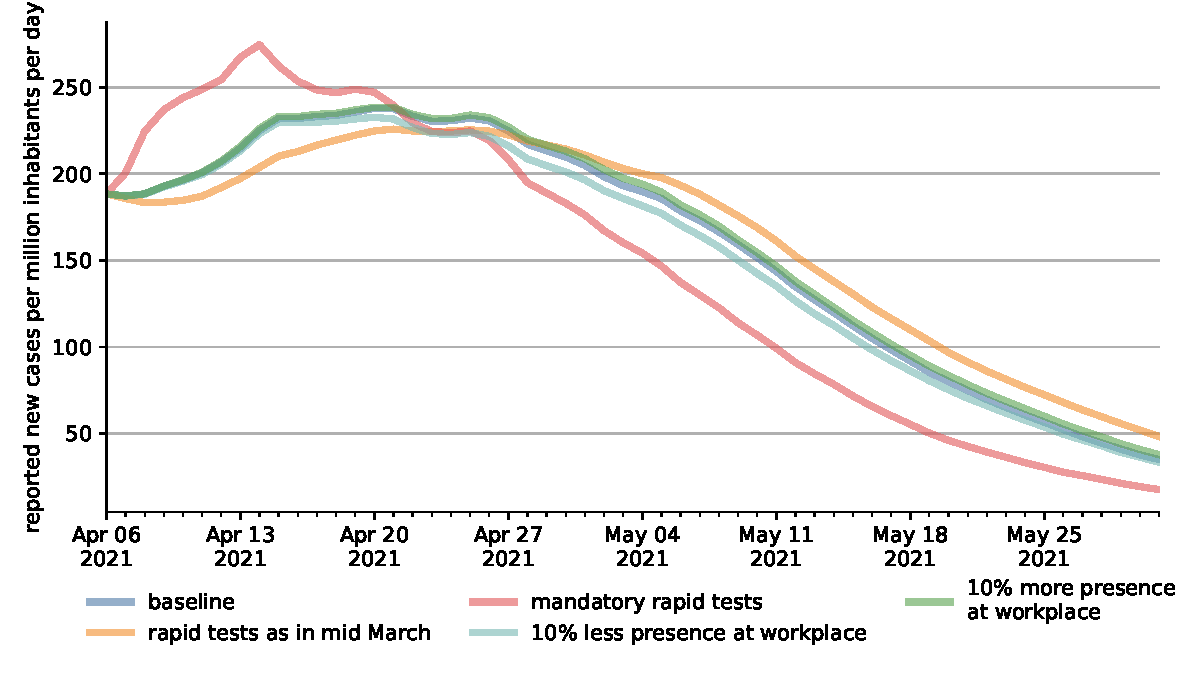
\includegraphics[width=0.9 \textwidth]{figures/results/figures/scenario_comparisons/new_work_scenarios/full_new_known_case}
    \caption{Reported Cases}
    \label{fig:work_scenarios_new_known_case}
  \end{subfigure}
  \hfill
  \begin{subfigure}[b]{.49\textwidth}
    \centering
    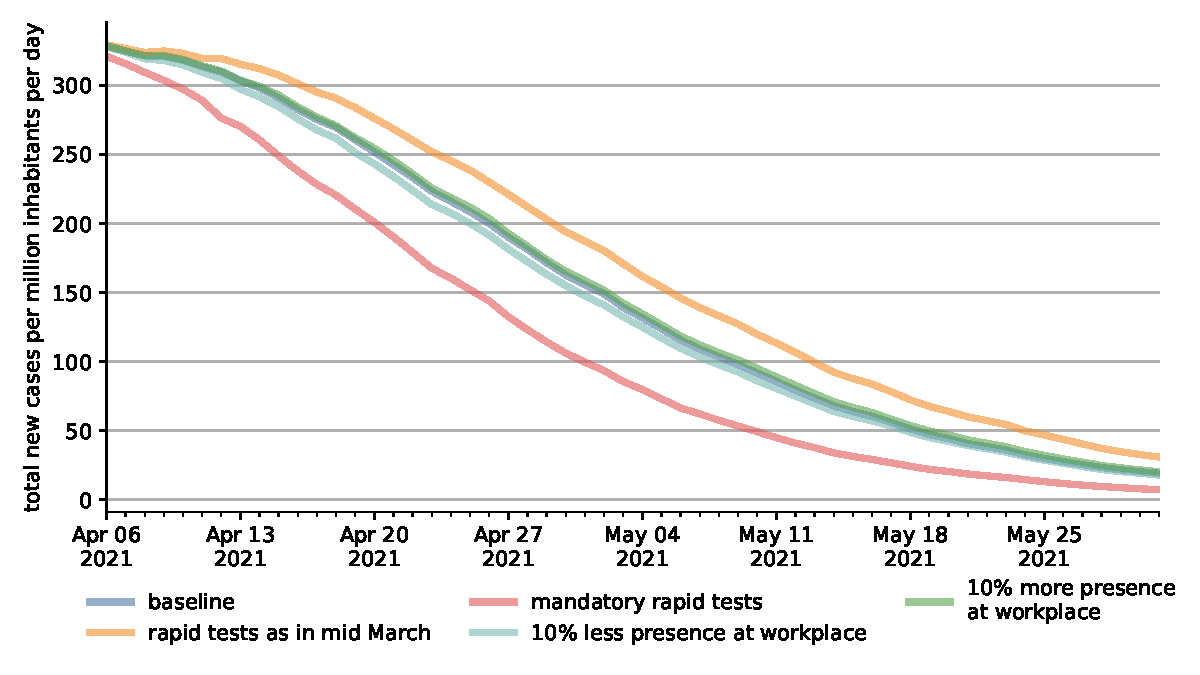
\includegraphics[width=0.9 \textwidth]{figures/results/figures/scenario_comparisons/new_work_scenarios/full_newly_infected}
    \caption{Total Cases}
    \label{fig:work_scenarios_newly_infected}
  \end{subfigure}
  \caption{The Effect of Different Work Scenarios on Reported and Total Cases}
  \label{fig:work_scenarios_detailed}
  \floatfoot{\noindent \textit{Note:} The figure shows the development of cases after
  different hypothetical work policy changes take place at Easter until the end of our
  simulation period. We vary the share of workers that have physical work contacts (10\%
  more or less compared to the share in the baseline scenario, 85\% or 70\% of workers,
  respectively) and how many tests are performed at work relative to our baseline
  scenario. As an ambitious scenario we implement mandatory tests for all employees that
  do not work from home, assuming 95\% compliance on both the employer and the employee
  side. On the other hand, we show what would have happened if the test offers had fallen
  back to the level of mid March (only 14\% of workers are tested regularly). The
  observed cases can be misleading because more testing leads to more detected cases. It
  takes two to three weeks for the reduction in new infections to dominate the increased
  detection. Furthermore, the two opposing effects lead to a smaller effect size than is
  actually the case.}
\end{figure}


\FloatBarrier

The second commonly employed and also very contentious NPI we look at are school
closures. Due to the very high incidence we model the German schooling policy as
generous emergency care with rotating on-site schooling for graduating classes for April.
In May where cases fall and schools gradually opened, we model the policy as
rotating on-site schooling for most students (except for children eligible for emergency
care and graduating classes who attend in full). We compare this baseline scenario to
simply keeping schools completely closed (the brown line) and opening schools normally
(but maintaining our hygiene multiplier to account for mask wearing, ventilation etc.)
with and without tests.

As can be seen, the transmission potential in schools is very low both in the generous
emergency setting as well as the rotating operation. The difference to keeping schools
completely closed is very small. Also, consistent testing reduces the transmission
potential at schools strongly. Had schools opened directly after Easter given the testing
rates Germany managed at schools during that time, the total incidence would have been
only been 9 incidence points higher on average. Tests, however, are crucial here. Had
schools opened completely without any testing of students and staff, schools would have
added up to 50 incidence points.

\begin{figure}[ht] % School Scenarios
  \centering
  \begin{subfigure}[b]{.49\textwidth}
    \centering
    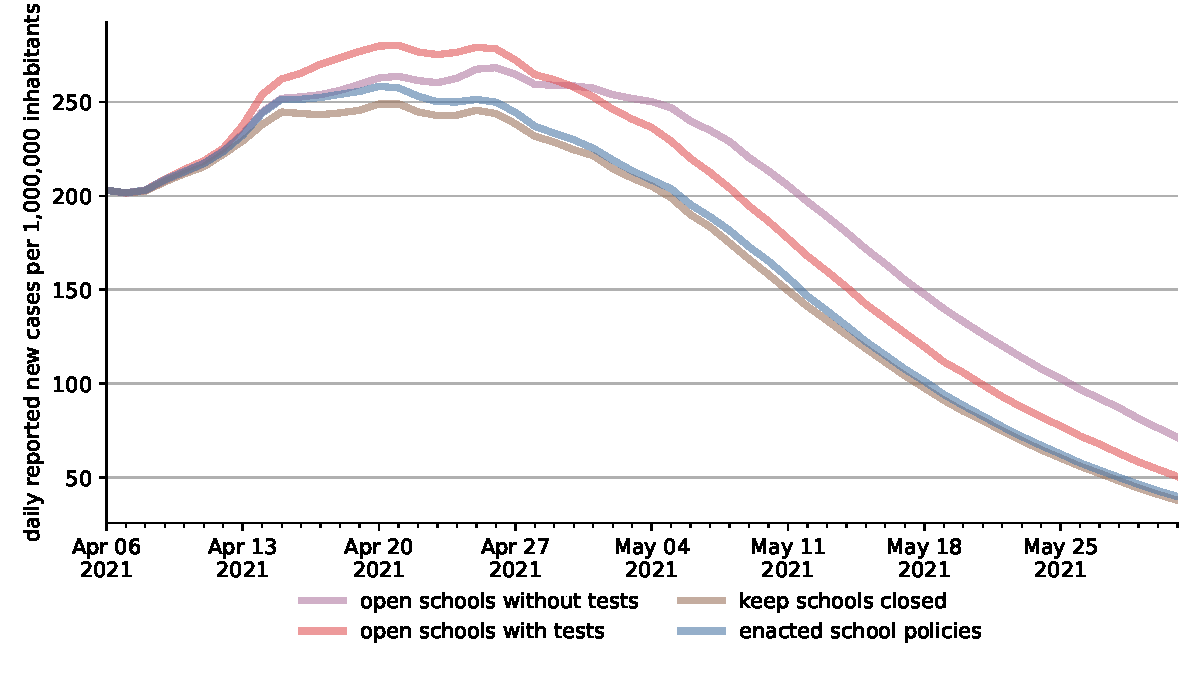
\includegraphics[width=0.9 \textwidth]{figures/results/figures/scenario_comparisons/school_scenarios/full_new_known_case}
    \caption{Reported Cases}
    \label{fig:school_scenarios_new_known_case}
  \end{subfigure}%
  \hfill
  \begin{subfigure}[b]{.49\textwidth}
    \centering
    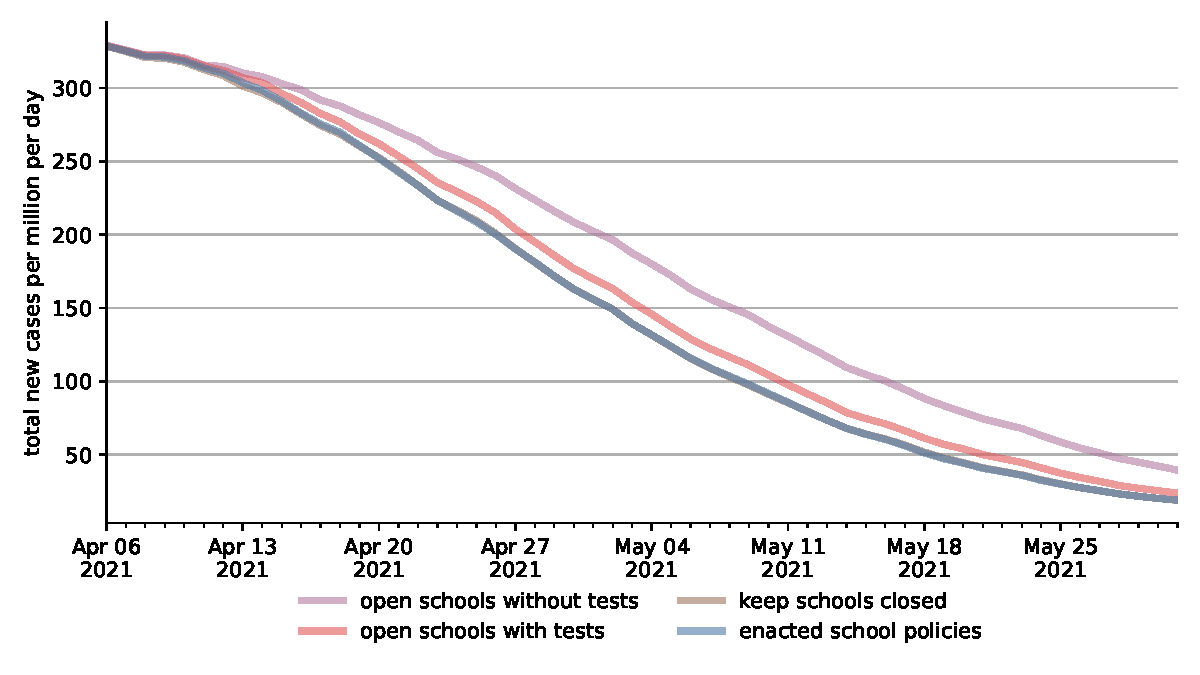
\includegraphics[width=0.9 \textwidth]{figures/results/figures/scenario_comparisons/school_scenarios/full_newly_infected}
    \caption{Total Cases}
    \label{fig:school_scenarios_newly_infected}
  \end{subfigure}
  \caption{The Effect of Different School Scenarios on Reported and Total Cases}
  \label{fig:school_scenarios_detailed}
  \floatfoot{\noindent \textit{Note:} The figure shows the development of cases after
   different hypothetical school policy changes take place at Easter until the end of our
   simulation period. Apart from the enacted school policies as our baseline we simulate
   how cases would have developed if schools had been closed completely as the strictest
   possible counterfactual scenario and two opening models: One where schools open
   normally (with hygiene measures) without any testing in the education sector and one
   where schools open normally but testing develops as in the baseline scenario.   %Our simulations suggest that the enacted policies were as effective as keeping schools
   %closed. Opening schools with the testing schemes that were in place after Easter would
   %have had a small effect on the overall incidence. However, this is mainly due to the
   %stringent testing that was in place in schools by that time. Had schools opened
   %without testing requirements the total incidence would have been up to 50 points
   %higher, though this would have been less visible in the reported cases.
   }
\end{figure}

\FloatBarrier

Lastly, we shed some light on the role our rapid test demand channels play
for the effect of rapid tests on case numbers. To do so we ran two scenarios where we
allocated rapid tests either completely randomly in the entire population or among 70\%
of the population to account for the fact that a share of the population might refuse or
be very hard to reach with rapid tests.\footnote{We calculate the number of rapid tests
as in our baseline model. This leads to similar numbers of rapid tests. However given the
higher incidence in our random scenarios these scenarios have a slightly higher number of
rapid tests.}

Figure \ref{fig:random_rapid_tests_detailed} shows how the incidence of detected and
total cases develops in the two random scenarios (red and purple line) relative to our
baseline scenario (blue line). Two things stand out: Firstly, the total number of cases
falls much faster in our baseline scenario compared to the two random scenarios.
Secondly, this is not because the share of detected cases is higher in the baseline
scenario; in fact, it is even slightly lower until end of April.

There are two mechanisms that can explain these surprising facts: Firstly, tests at the
workplace predominantly target a group that has many contacts. Thus, catching infections
in this group prevents more infections than in the general population. Secondly, rapid
tests that are done because of private contact tracing are more effective at interrupting
infection chains because they catch many infections in an early stage. Isolating infected
individuals early on means that there are fewer days on which they can infect others.
%
The difference between the two random scenarios are small. This is likely due to only a
small fraction of the population being tested on any given day.


\begin{figure}[ht] % Random Rapid Tests
  \centering
  \begin{subfigure}[b]{.49\textwidth}
    \centering
    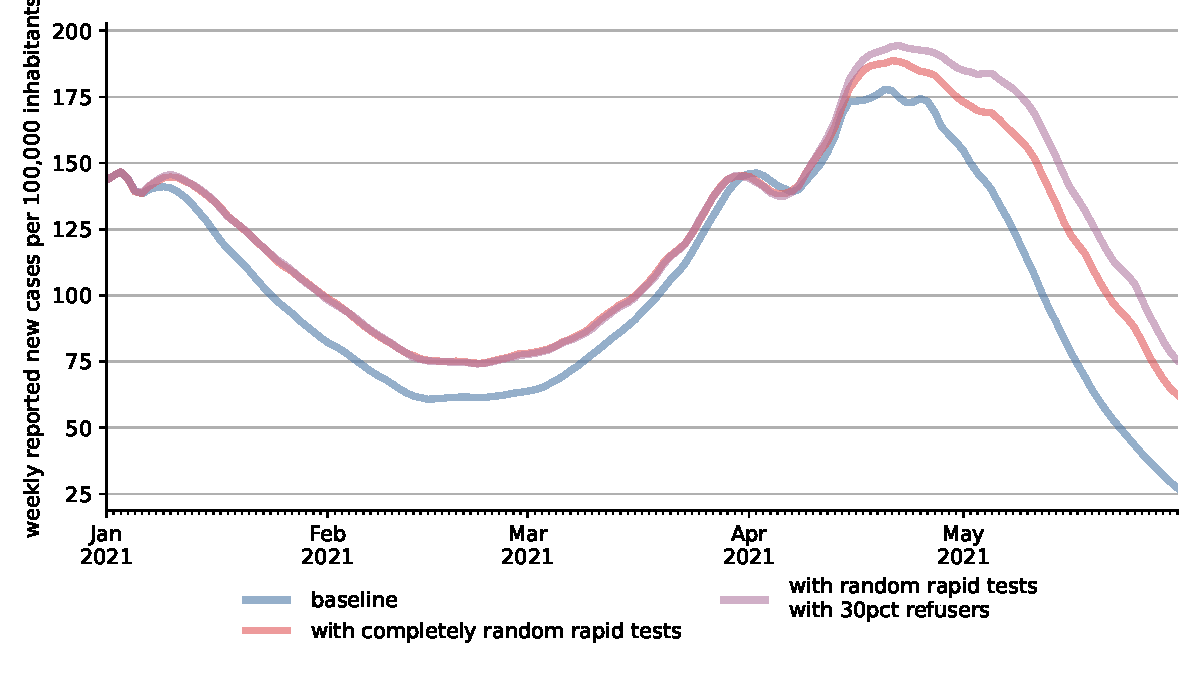
\includegraphics[width=0.9 \textwidth]{figures/results/figures/scenario_comparisons/random_rapid_tests_vs_baseline/full_new_known_case}
    \caption{Reported Cases}
    \label{fig:random_rapid_tests_new_known_case}
  \end{subfigure}%
  \hfill
  \begin{subfigure}[b]{.49\textwidth}
    \centering
    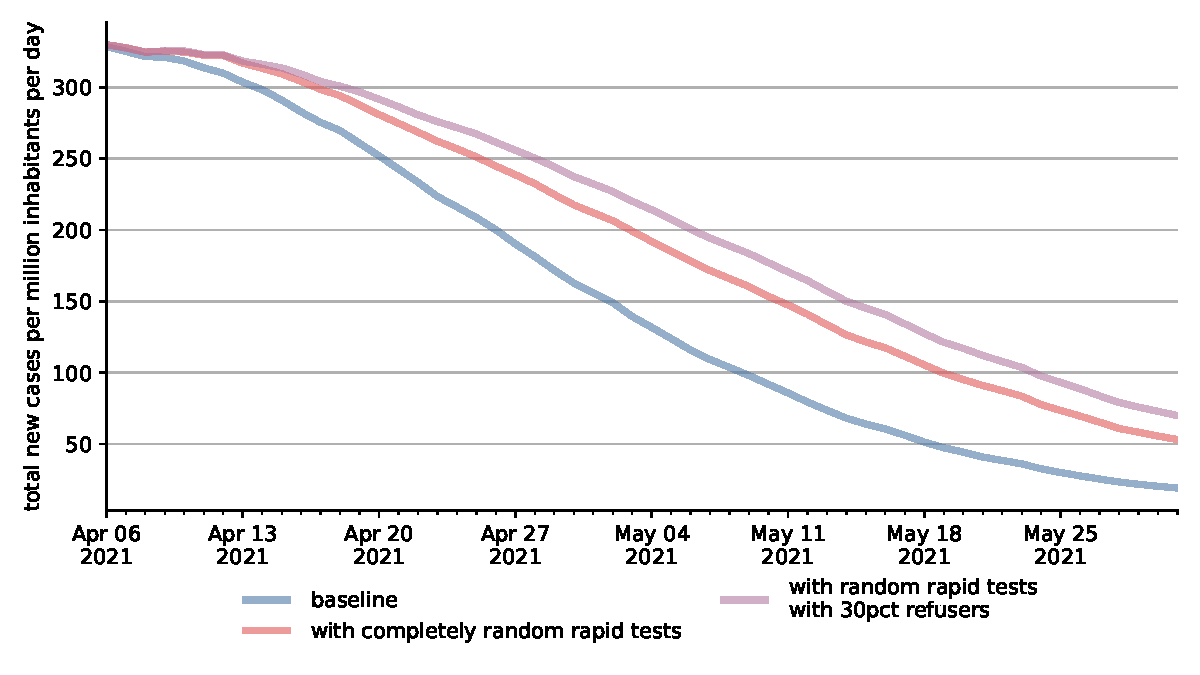
\includegraphics[width=0.9 \textwidth]{figures/results/figures/scenario_comparisons/random_rapid_tests_vs_baseline/full_newly_infected}
    \caption{Total Cases}
    \label{fig:random_rapid_tests_newly_infected}
  \end{subfigure}

  \caption{The Role of Targeted and Compliance Driven Rapid Test Demand}
  \label{fig:random_rapid_tests_detailed}

  \floatfoot{\noindent \textit{Note:} The figure shows the development of cases in two
  scenarios where rapid tests are distributed randomly in the population compared to our
  baseline scenario after Easter. In the baseline scenario rapid tests are targeted to
  workers, students, teachers and individuals at high risk of being infected including a
  weekly or twice weekly spacing between rapid tests. In the scenario with 30\% refusers
  tests are randomly distributed among 70\% of the population who are identified as
  compliers.
  }
\end{figure}

\FloatBarrier
